\chapter{Theoretische methodes}

	\par Een probleem dat zich kan voordoen bij de ge\"implementeerde methode is dat ook de kleur van andere blauwe objecten gewijzigd wordt. Wanneer het blauw eenmaal binnen de ingestelde grenzen valt zal het van kleur veranderd worden. Om dit probleem op te lossen kan gebruik gemaakt worden van een techniek die het mogelijk maakt om objecten realtime in video te herkennen. Wanneer er dan een smurf op het beeldfragment herkend wordt zal enkel dit deel van het beeldfragment een koerswijziging ondergaan. Deze techniek brengt ook onmiddellijk een tweede voordeel met zich mee omdat niet elk beeld volledig, pixel per pixel, overlopen dient te worden om na te gaan of de pixel binnen de ingestelde kleurgrenzen past. 

	\par Wanneer men enkel werkt met de intensiteit van een pixel (RGB, YUV, YCbCr\ldots) dan wordt dit naar aantal bewerkingen vaak groot en zwaar voor de processor wanneer men elke pixel \'e\'en voor \'e\'en moet doorlopen. Dit vormt een probleem wanneer er gebruik gemaakt wordt van realtime video. Om het aantal processor instructies te reduceren is dus een andere techniek nodig. Het gebruik van wavelets biedt een oplossing voor bovenstaand probleem, en maakt het tevens ook mogelijk om de objectdetectie uit te voeren.

	\par Een andere weg die gevolgd kan worden is om wel pixel-per-pixel te werken maar de datastroom op een andere manier aan de processor aan te bieden. In de huidige implementatie wordt telkens een beeld opgevraagd uit het level 3 geheugen van de processor. Dit is een zeer dure operatie wat betreft instructies. Door slim om te springen met de DMA-controller kan men de toevoer van data versnellen en zo het aantal instructies aanzienlijk verminderen. 

\section{Objectdetectie aan de hand van Haar-like-features}

	\par Een relatief eenvoudige techniek die gebruikt wordt om objecten te detecteren is de haar-cascade. Deze techniek maakt gebruik van Haar-like-features om objecten te detecteren. Een ge\"isoleerde pixel bevat enkel informatie over de luminantie en kleur van die bepaalde pixel. Het vertelt niets meer over de structuur of het uitzicht van het geheel. Om meer informatie te krijgen over het geheel dient men een aantal aangrenzende pixels te aanschouwen als een verzameling. Het Viola-Jones algoritme is een feature-based algoritme dat in tegenstelling tot een pixel-based algoritme gebruik maakt van features om objecten te detecteren. Het algoritme maakt gebruik van Haar wavelets. Dit type wavelet laat toe om visuele patronen te beschrijven als een luminantieverandering op verschillende frequenties.

	\par Het Viola-Jones algoritme is ook zelflerend en kan getraind worden door middel van een oefenset afbeeldingen die zowel positieve als negatieve afbeeldingen bevat. zo$'$n model wordt een classificator genoemd en bestaat typisch uit enkele honderdtallen positieve en enkele negatieve afbeeldingen.

	\par Om een classificator aan te maken, wat ook wel training van een classificator genoemd wordt, wordt een wavelet transformatie uitgevoerd op de trainingsafbeelding aan de hand van een haar-like-feature. Om dit proces te versnellen wordt niet de originele afbeelding gebruikt, maar de integraalafbeelding. Een integraalafbeelding kan als volgt gegenereerd worden. De waarde van de pixel op positie x,y van de integraalafbeelding is gelijk aan de waarden van alle pixels met kleinere x- en y-waarden op de originele afbeelding. Vervolgens zullen de pixels van de integraalafbeelding getest worden door middel van een venster dat over de integraalafbeelding heenschuift. Elke feature heeft na deze fase een bepaalde wegingsfactor. Een geheel van deze wegingsfactoren omschrijft dan op zijn beurt een bepaald object.

	\par De integraalafbeelding wordt getest met de haar-like features die weergegeven zijn in figuur~\ref{fig:HaarFeatureImage} op pagina ~\pageref{fig:HaarFeatureImage}. Afhankelijk van de vereiste nauwkeurigheid zal al dan niet de hele set overlopen worden. Dit wordt ook wel eens haar-cascade genoemd. Een model bestaat dus uit een aaneenschakeling van verschillende haar-like-features. 

		\begin{figure}[H]
			\centering
			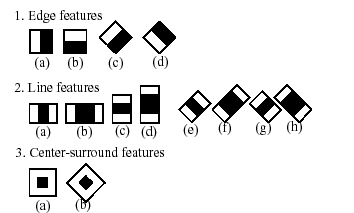
\includegraphics[width=0.65\textwidth]{Chapters/Chapter3/Images/haarfeatures.png}
			\caption{Set van haar-like features die gebruikt worden voor objectdetectie (Bron: http://docs.opencv.org)}
			\label{fig:HaarFeatureImage}
		\end{figure}

	\par Het Viola-Jones algoritme maakt gebruik van bovenstaand model dat opgebouwd is uit haar-like-features om te evalueren of een inkomend beeld het te detecteren object bevat. Alvorens de wavelet op een beeldfragment wordt toegepast, zal eerst een luminantie normalisatie doorgevoerd worden. Hierna zal het beeld verkleind worden tot een resolutie om het verwerkingsproces te versnellen. Vervolgens zal de wavlettransformatie van de afbeelding, die analoog verloopt met het trainen van een model, doorlopen worden en vergeleken worden met het model om zo te evalueren of het te detecteren object op de afbeelding staat. Vervolgens kan ook de positie en grootte (onder de vorm van een rechthoekig gebied) weergegeven worden. 

	\par Wanneer er dus een smurf op de afbeelding gedetecteerd word dan pas dient er op het gedeelte van waar de smurf gedetecteerd is een kleurverandering toegepast te worden. Die detectie van smurfen kan uitgevoerd worden door Core A en de effectieve kleursverandering kan uitgevoerd worden door Core B.

	\par Bovenstaand algoritme is relatief eenvoudig te implementeren op de BlackFin processor omdat de BlackFin Image Processing Toolbox een reeks tools bevat die speciefiek ontworpen zijn om Haar-features toe te passen. Deze toolbox is qua werking en opzet te vergelijken met de OpenCV bibliotheek. 

\section{Slim omspringen met de DMA-controller}
\label{sec:dmacontroller}
	\par Bij de huidige implementatie van de kleurverandering wordt een inkomend beeld telkens opgehaald vanuit het level 3 geheugen. E\'en beeld heeft ongeveer een grootte van 1 \'a 2 MB. Met een beschikbaar geheugen van 64 MB SDRAM kunnen er dus maximum 32 frames gebufferd worden in het SDRAM. De BlackFin beschikt zelf over 32 kB level 1 cache geheugen en 128 kB level 2 cache geheugen. Het voordeel aan dit level 1 en 2 geheugen is dat zij veel sneller aanspreekbaar zijn door de processor dan het relatief trage level 3 geheugen. 

	\par Er valt op te merken dat een volledig frame niet past in het level 1 of 2 geheugen van de BlackFin. Het zou wel mogelijk zijn om een deel van een frame te verplaatsen naar het level 1 of 2 geheugen, dit te verwerken en vervolgens het resultaat weer verplaatsen naar het level 3 geheugen. Deze acties kunnen volbracht worden door de DMA-controller waardoor er geen processorkracht nodig is om deze verplaatsing teweeg te brengen. Dit principe heeft een groot voordeel qua tijd omdat de processor zich enkel moet bezighouden met het bewerken van data, en niet het opvragen ervan. 

	\par Wanneer men de frame-informatie door middel van de DMA lijn per lijn naar het level 2 geheugen kan verplaatsen heeft te processor minder tijd nodig om een lijn te verwerken. Wanneer een lijn eenmaal verwerkt is wordt deze terug naar het level 3 geheugen gestuurd door middel van de DMA-controller. Op deze manier kan mits een aanpassing van de DMA-controller toch de huidige werkwijze van kleurverandering behouden blijven en er toch een grote snelheidswinst geboekt worden. Dit zal een aanzienlijke verbetering van de framerate teweegbrengen.
